%===================================================================
\chapter{Collisions}\label{chap.collision}

\section{Pitch-angle Scattering Operator}

The treatment of collisions in gyrokinetic simulations is not 
as intricate as that required in neoclassical simulations.
In the former case, the dominant effect of collisions is 
pitch-angle scattering in the electron equation.  Below we 
outline the implementation of this effect, and of the 
associated ion pitch-angle scattering operators.

\newcommand\apn{\delta A_{\parallel,n}}
\newcommand\apndot{\delta \dot{A}_{\parallel,n}}
\newcommand\fn{f_{\si,n}}

Treating the collision operator $\hat{C}$ by operator splitting 
leaves us with the following evolution equation 
%
\begin{equation}
\frac{\partial\hn}{\partial\hat{t}} = 
 \hat{C}\left[\hn - z_\si \alpha_\si \vphat \gav_\si \apn \right] \; .
\label{eq.c1}
\end{equation}
%
This has the alternative form
\begin{equation}
\frac{\partial\fn}{\partial\hat{t}} + z_\si \alpha_\si \vphat 
 \gav_\si \apndot = \hat{C}\left[\fn \right] \; ,
\label{eq.c2}
\end{equation}
%
where
%
\begin{equation}
\fn = \hn - z_\si \alpha_\si \vphat \gav_\si \apn \; . 
\end{equation}
%
We must take care to avoid the Amp\`ere cancellation problem
when solving this equation.  Furthermore, due to the viscous 
Courant limit on the timestep imposed by the operator $\hat{C}$ 
near the trapped-passing boundary, we use an implicit technique.
For typical time steps and 8-point pitch-angle grids, it appears 
that we are probably very close to the explicit stability limit 
at $\nu_{ei} \sim c_s/a$. Multiplying Eq.~(\ref{eq.c1}) by 
$z_\si \vphat$, summing over species and integrating gives 
%
\begin{equation}
-\frac{2\rhou^2}{\betau} \nabla_\perp^2 \apndot + 
\sum_\si \alpha_\si z_\si^2 \, \vop[\vphat^2 \gav^2_\si\apndot] = 
 \sum_\si z_\si  
 \vop\left[ \vphat \hat{C} \left[ \gav_\si \fn \right] \right] \; .
\end{equation}
%
It is sufficiently accurate to take $\hat{C}$ to be the pitch-angle 
scattering operator 
% 
\begin{equation}
\hat{C} = \hat{\nu}_\si \frac{\partial}{\partial \xi}
(1-\xi^2) \frac{\partial}{\partial\xi} \; ,
\end{equation}
%
with the corresponding identity
%
\begin{equation}
\vop\left[ \xi \hat{C} f \right] 
 = - 2 \hat{\nu}_\si \, \vop\left[ \xi f \right]  \; .
\end{equation}
%
For ions, it is convenient, and probably more realistic physically, 
to assume that $\hat{C}$ also conserves momentum, so that 
%
\begin{equation}
\vop[ \xi \hat{C} f ] = 0 \; .
\end{equation}
%
We can write the following equation for $\dapdot = \partial\dap/\partial t$:
%
\begin{equation}
{\cal L}_A \apndot = \vop\left[ 2 \hat{v}_{\parallel,e} \hat{\nu}_\e f_{\e,n} 
\right] \; .
\end{equation}
%
Then, we solve Eq.~(\ref{eq.c2}) with a semi-implicit advance
%
\begin{align}
\left( 1- \hat{C} \Delta t \right) \bar{f}_{\si,n} 
 &~= \fn - z_\si \alpha_\si \vphat \gav_\si \apndot \Delta t \; , \\
 &~= \hn - z_\si \alpha_\si \vphat \gav_\si (\apn + \apndot \Delta t) \; .
\end{align}
%
Currently, in GYRO, we set $\gav_\si = 1$ in the final equation, 
since the ion collisional effects are weak and already rather 
approximate.

\subsection{The Radial Basis Function (RBF) Method}

We are interested in developing a method of function approximation 
suitable for evaluating differential and integral operators on 
an irregular mesh in the $(\theta,\xi)$ plane.  The mesh itself
is determined by features of the collisionless dynamics and 
cannot be altered to suit the evaluation of the collision 
operator.  We will formulate the problem such that the 
$\theta$-dependence is periodic on the interval $-\pi \le \theta < \pi$.
In the $\xi$ domain, there are no boundary conditions (only
regularity of the solution) on the interval $-1 \le \xi \le 1$. 

%====================================================================
\begin{figure}[h]
\begin{center}
\includegraphics[scale=0.7]{figures/stencil.ps}
\caption{Irregular mesh in the $(\theta,\xi)$-plane.}
\label{fig.stencil}
\end{center}
\end{figure}
%===================================================================

In reality the functions to be approximated is not in general
a periodic function of $\theta$, but rather satisfied a phase 
condition of the type $f(\theta+2\pi) = f(\theta) e^{2\pi i \alpha}$.
Since it is highly desireable to approximate a periodic 
function to eliminate boundary-related headaches, one can 
instead consider the associated function 
$g(\theta) = f(\theta) e^{-i \alpha  \theta}$, which is periodic.
 
\subsection{Basic RBF expansion}

\newcommand\xv{{\bf x}}
\newcommand\xc{{\hat {\bf x}}}
\newcommand\xih{{\hat\xi}}

We start by briefly describing the basic RBF approximation.
Given a function $\phi(r)$, $r \ge 0$, {\it centers} 
$\xv_1,\ldots,\xv_N$, and data $f_i = f(\xv_i)$, the basic 
form of the RBF approximation is
%
\begin{equation}
F(\xv) = \sum_{i=1}^N c_i \phi(|\xv-\xv_i|) \; ,
\label{eq.basicrbf}
\end{equation}
%
where $|\cdot|$ is a positive-definite norm on the vector 
space of interest.  The $c_i$ are then chosen so that 
$F(\xv_i) = f_i$.  Typical RBF choices are 

%====================================================================
\begin{table}[h]
\begin{center}
\caption{Typical basis functions}
\begin{tabular}{c c c} \hline\hline
 $\phi(r)$ & name & smoothness \\ \hline
 $r^3$ & cubic RBF & piecewise smooth \\ 
 $r^5$ & quintic RBF & piecewise smooth \\ 
 $r^2 \log r$ & thin-plate spline & piecewise smooth \\ 
 $\sqrt{1+(\epsilon r)^2}$ & multiquadric & infinitely smooth \\ 
 $e^{-(\epsilon r)^2}$ & Gaussian & infinitely smooth \\ 
\hline\hline
\end{tabular}
\label{tab.error}
\end{center}
\end{table}
%====================================================================

In practice, the infinitely smooth RBFs are difficult to use 
because the associated coefficient matrices $A_{ij} = \phi(|\xv_j-\xv_i|)$ 
are notoriously ill-conditioned in the limit $\epsilon \rightarrow 0$, 
although theoretically they are capable of spectral convergence 
and thus remarkably accurate approximation in this limit.  Testing, 
nevertheless indicates that the cubic and quintic RBFs are much 
more robust and therefore appropriate for the mesh sizes of interest 
in the collision problem.  In one dimension, there is a simple 
relationship between cubic and quntic RBFs and cubic and quintic 
$B$-splines.  Thus, the remedy for boundary inaccuracy is one that 
is already known from the theory of spline interpolation. 

\subsection{Influence of boundaries}

It is well-known that near boundaries, the accuracy of RBF 
approximation -- like all function approximation near boundaries -- 
can suffer a significant loss of accuracy, and can lead to 
stability problems when used for operator discretization in 
time-dependent problems.  We have indeed verified that accuracy 
loss at the boundary is a serious issue in the $\xi$ direction.

Curing the boundary instability problem first requires generalizing 
somewhat the RBF expansion in Eq.~(\ref{eq.basicrbf}).  We need to 
allow the locations of the centers to deviate in some cases from 
the locations of the fixed mesh points -- even allowing them to 
move outside the simulation domain $-1 \le \xi \le 1$.  So, we
write
%
\begin{equation}
F(\xv) = \sum_{i=1}^N c_i \phi(|\xv-\xc_i|) \; ,
\label{eq.rbf}
\end{equation}
%
where as before the $c_i$ are chosen so that 
$F(\xv_i) = f_i$.  Mesh points $\xv_i$ near the boundaries at 
$\xi = \pm 1$ are moved outside the boundary in an analog of
the Super Not-a-Knot (SNaK) approach.

\subsection{The method in detail}

The domain of interest is topologically equivalent to 
the surface of a cylinder, so there is a natural the 
distance function 
%
\begin{equation}
r_i = |\xv-\xc_i| = \sqrt{2-2\cos(\theta-\theta_i)+(\xi-\xih_i)^2}
\end{equation}
%
For $s=3,5,\ldots$, we write
%
\begin{equation}
\phi(r_i) = r_i^s \doteq R_0(\theta-\theta_i,\xi-\xih_i;s) 
\end{equation}
%
\begin{equation}
\frac{\partial}{\partial\xi} \phi(r_i) 
 = s r_i^{s-2} (\xi-\xih_i) 
\doteq R_1(\xi-\xih_i,\theta-\theta_i;s)
\end{equation}
%
\begin{equation}
\frac{\partial^2}{\partial\xi^2} \phi(r_i) 
 = r_i^{s-4} \left[ s(s-2)(\xi-\xih_i)^2 + s r_i^2 \right] 
\doteq R_2(\xi-\xih_i,\theta-\theta_i;s)
\end{equation}
%
\begin{align}
{\cal L} f = &~\frac{\partial}{\partial\xi} (1-\xi^2)
\frac{\partial}{\partial \xi} f(\theta,\xi) \\
= &~(1-\xi^2) \sum_i c_i R_1(\xi-\xih_i,\theta-\theta_i;s) 
- 2\xi \sum_i c_i R_2(\xi-\xih_i,\theta-\theta_i;s) \\
\doteq &~\sum_i c_i L(\theta,\xi,\theta_i,\xih_i)
\end{align}
%
Thus, in matrix notation, we can write
%
\begin{equation}
({\cal L} f)_i = L_{ij} c_j = L_{ij} (R_0^{-1})_{jk} f_k \doteq D_{ik} f_k
\end{equation}
%
The matrices are
%
\begin{align}
L_{ij} = &~L(\theta_i,\xi_i,\theta_j,\xih_j) \\
(R_0)_{ij} = &~R_0(\theta_i-\theta_j,\xi_i-\xih_j;s)
\end{align}
%
Implementation of the Crank-Nicholson scheme for the equation
%
\begin{equation}
\frac{\partial f}{\partial t} = \nu {\cal L} f
\end{equation}
%
is then written as
%
\begin{align}
f_i(t+\Delta t) = &~\left( 1-\frac{\nu \Delta t}{2} D \right)_{ij}^{-1}
\left( 1+\frac{\nu \Delta t}{2} D \right)_{jk} f_k(t) \\
\doteq &~M_{ik} f_k(t)
\end{align}
%
In GYRO, we compute and store the matrix $M$ at start-up,
reducing the collision step to a matrix-vector multiply.
The drawback of course is the storage, which is significant
for a matrix of this type.

\subsection{Additional comments}

For a fixed number of meshpoints, the condition number of the 
matrix $(R_0)_{ij}$ grows rapidly.  So, although the method is 
mathematically correct for $s=3,5,7,\ldots$, in practice the 
scheme is probably limited to $s=3$ and $5$.

\section{Conservative Krook Operator}

The operator is an annhiliation term $-\nu f$ plus a 
restoring term $\delta C$.
%
\begin{equation}
C f = -\nu f + \delta C 
\end{equation}
%
\begin{equation}
\mbox{{\sc number}:} \qquad \fvop \left[ F_m^*(\theta) \delta C \right] 
= \fvop \left[ F_m^*(\theta) \nu f \right] \doteq S_m^{(1)}
\end{equation}
\begin{equation}
\mbox{{\sc momentum}:} \qquad \fvop 
 \left[ F_m^*(\theta) \vp \delta C \right] 
= \fvop \left[ F_m^*(\theta) \vp \nu f \right] \doteq S_m^{(2)}
\end{equation}
\begin{equation}
\mbox{{\sc energy}:} \qquad \fvop \left[ F_m^*(\theta) 
 \ehat \delta C \right] 
= \fvop \left[ F_m^*(\theta) \ehat \nu f \right] \doteq S_m^{(3)}
\end{equation}

\noindent
To determine the restoring term, expand
%
\begin{equation}
\delta C = \sum_m c_m^1 F_m(\theta)
+ \vp(\theta)\sum_m c_m^2 F_m(\theta) 
+ \ehat \sum_m c_m^3 F_m(\theta) 
\end{equation}

\noindent
Now we must determine each $c_m$ as a function of the $S_m$.
%
\begin{align}
A^{11}_{m\mpr} c^1_{\mpr} + A^{13}_{m\mpr} c^3_{\mpr} = &~S_m^{(1)} \\
                          A^{22}_{m\mpr} c^2_{\mpr} = &~S_m^{(2)} \\
A^{31}_{m\mpr} c^1_{\mpr} + A^{33}_{m\mpr} c^3_{\mpr} = &~S_m^{(3)}
\end{align}

where

\begin{align}
A^{11}_{m\mpr} = &~\fvop\left[ F_m^* F_\mpr \right] \\
A^{13}_{m\mpr} = &~\fvop\left[ F_m^* \ehat F_\mpr \right] \\
A^{31}_{m\mpr} = &~\fvop\left[ F_m^* \ehat F_\mpr \right] = A^{13}_{m\mpr} \\
A^{33}_{m\mpr} = &~\fvop\left[ F_m^* \ehat^2 F_\mpr \right] \\
A^{22}_{m\mpr} = &~\fvop\left[ F_m^* \vp^2 F_\mpr \right]
\end{align}
